\chapter{Конструкторская часть}

В данном разделе представлены математические основы алгоритма обратной трассировки лучей, разработка алгоритма обратной трассировки лучей и разработка типов и структур данных.

\section{Математические основы алгоритма обратной трассировки лучей}

\subsection{Поиск пересечения луча с полигонами}

Для поиска пересечения луча с полигонами используется барицентрический тест \cite{triangleintersection}. Это самый известный тест на пересечение <<луч-треугольник>>. Имея три точки на плоскости, можно выразить любую другую точку через ее барицентрические координаты.

Пусть луч $R(t)$ с началом в точке $O$ и нормализованным вектором направления $D$ определяется как:
\begin{equation}
	R(t) = O + tD
\end{equation}

Пусть вершины полигона обозначаются как $V_0, V_1, V_2$
Тогда, точка $T(u,v)$ в полигоне задаётся выражением:
\begin{equation}
	T(u,v) = (1 - u - v)V_0 + uV_1 + vV_2,
\end{equation}
где $(u,v)$ -- барицентрические координаты ($u \geq 0, v \geq 0, u + v \leq 1$)

Вычисление пересечения луча $R(t)$ и треугольника эквивалентно решению уравнения
$R(t) = T(u, v)$. В этом случае получим:
\begin{equation}
	O + tD = (1- u - v)V_0 + uV_1 + vV_2
\end{equation}

В матричном виде:
\begin{equation}
\label{slau}
\begin{bmatrix}
	-D & V_1 - V_0, V_2 - V_0
\end{bmatrix}
\begin{bmatrix}
t\\
u\\
v
\end{bmatrix} = O - V_0 
\end{equation}

Это означает, что барицентрические координаты ($u,v$) и расстояние $t$ от точки испускания луча до точки пересечения луча с полигоном могут быть найдены путём решения СЛАУ (системы линейных алгебраических уравнений), которая написана выше.

Вышесказанное можно рассматривать геометрически как перевод полигона (треугольника) в начало координат и преобразование его в в треугольник с единичными длинами по $y$ и $z$ с направлением луча по оси $x$. Это показано на рисунке
\ref{img:intersection}.

\begin{table}[H]
	\centering
	\begin{tabular}{p{1\linewidth}}
		\centering
		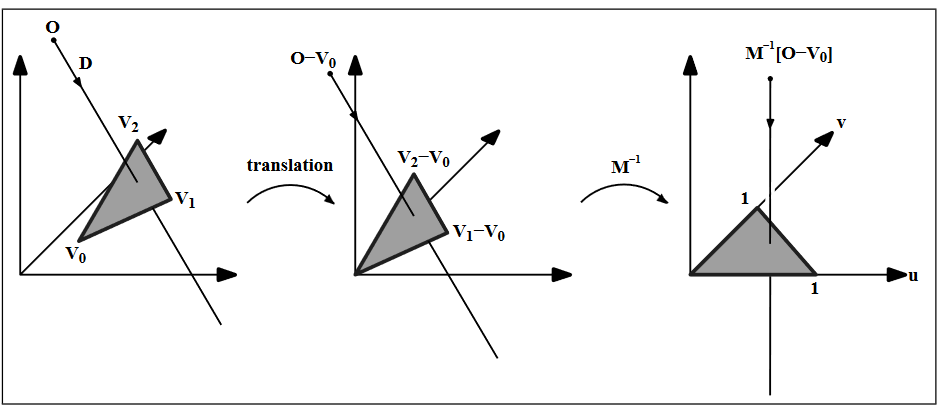
\includegraphics[width=0.9\linewidth]{include/intersection.png}
		\captionof{figure}{Иллюстрация для расчёта отражённого луча}
		\label{img:intersection}
	\end{tabular}
\end{table}


Пусть $E_1=V_1-V_0, E_2=V_2-V_0$ и $T=O - V_0$. Тогда, используя метод Крамера для (\ref{slau}):

\begin{equation}
\label{solution}
\begin{bmatrix}
t\\
u\\
v
\end{bmatrix} = \frac{1}{(D\times E_2) \cdot E_1}
\begin{bmatrix}
(T\times E_1) \cdot E_2\\
(D\times E_2) \cdot T\\
(T\times E_1) \cdot D
\end{bmatrix} = \frac{1}{P \cdot E_1}
\begin{bmatrix}
Q \cdot E_2\\
P \cdot T\\
Q \cdot D
\end{bmatrix},
\end{equation}
где $P = D \times E_2$ и $Q = T \times E_1$.

\subsection{Поиск нормали к полигонам}

Для поиска нормали к полигонам необходимо найти векторное произведение двух векторов, которые лежат на полигоне:
\begin{equation}
N = (V_2 - V_0) \times (V_1 - V_0),
\end{equation}
где $V_0, V_1, V_2$ -- вершины полигона.

\subsection{Поиск направления преломлённого и отражённого лучей}

Для алгоритма обратной трассировки лучей нужно уметь находить отражённый и преломлённый лучи, при этом учитывая модель освещения Уиттеда.
Отражённый луч можно найти, зная направление падающего луча и нормаль к поверхности. 

Пусть $L$ -- направление луча, а $n$ -- нормаль к поверхности. 
Луч можно разбить на две части: $L_p$ которая перпендикулярна нормали, и  $L_n$ – параллельна нормали.

Представленная ситуация изображена на рисунке \ref{img:illustation}.

\begin{table}[H]
	\centering
	\begin{tabular}{p{1\linewidth}}
		\centering
		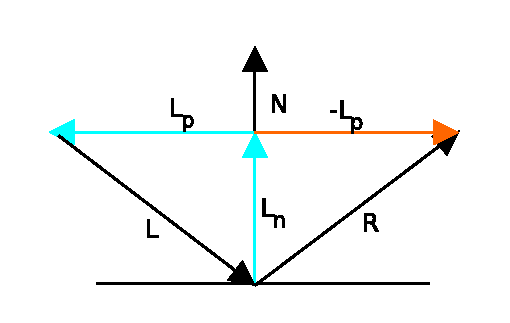
\includegraphics[width=0.7\linewidth]{include/illustation.pdf}
		\captionof{figure}{Иллюстрация для расчёта отражённого луча}
		\label{img:illustation}
	\end{tabular}
\end{table}

Учитывая свойства скалярного произведения $L_n = n \cdot (n, L)$ и  $L_p = L - n \cdot (n,L)$
Так как отражённый луч выражается через разность этих векторов, то отражённый луч выражается по формуле (\ref{reflect_ray}):
\begin{equation}
\label{reflect_ray}
R = 2 n \cdot (n, L) - L
\end{equation}

По закону преломления падающий, преломлённый лучи и нормаль к поверхности лежат в одной плоскости. 
Пусть $\{\mu_i\}$ -- показатели преломления сред, а $\{\eta_i\}$ – углы падения и отражения света соответственно. 
Применяя закон Снеллиуса, параметры преломлённого луча можно вычислить по формуле (\ref{refract_ray}):
\begin{equation}
\label{refract_ray}
\begin{aligned}
R = \frac{\mu_1}{\mu_2} L + ( \frac{\mu_1}{\mu_2} \cos(\eta_1) - \cos(\eta_2))n ,
\end{aligned}
\end{equation} 
где $\cos(\eta_2) = \sqrt{1 - (\frac{\mu_1}{\mu_2})^2 \cdot (1 - \cos(\eta_1))^2}$

\section{Разработка алгоритма обратной трассировки лучей}

На рисунках \ref{img:r1} -- \ref{img:r4} представлены схемы алгоритма испускания луча и алгоритмов поиска пересечения луча со сценой, с объектом и с полигоном.

\begin{table}[H]
	\centering
	\begin{tabular}{p{1\linewidth}}
		\centering
		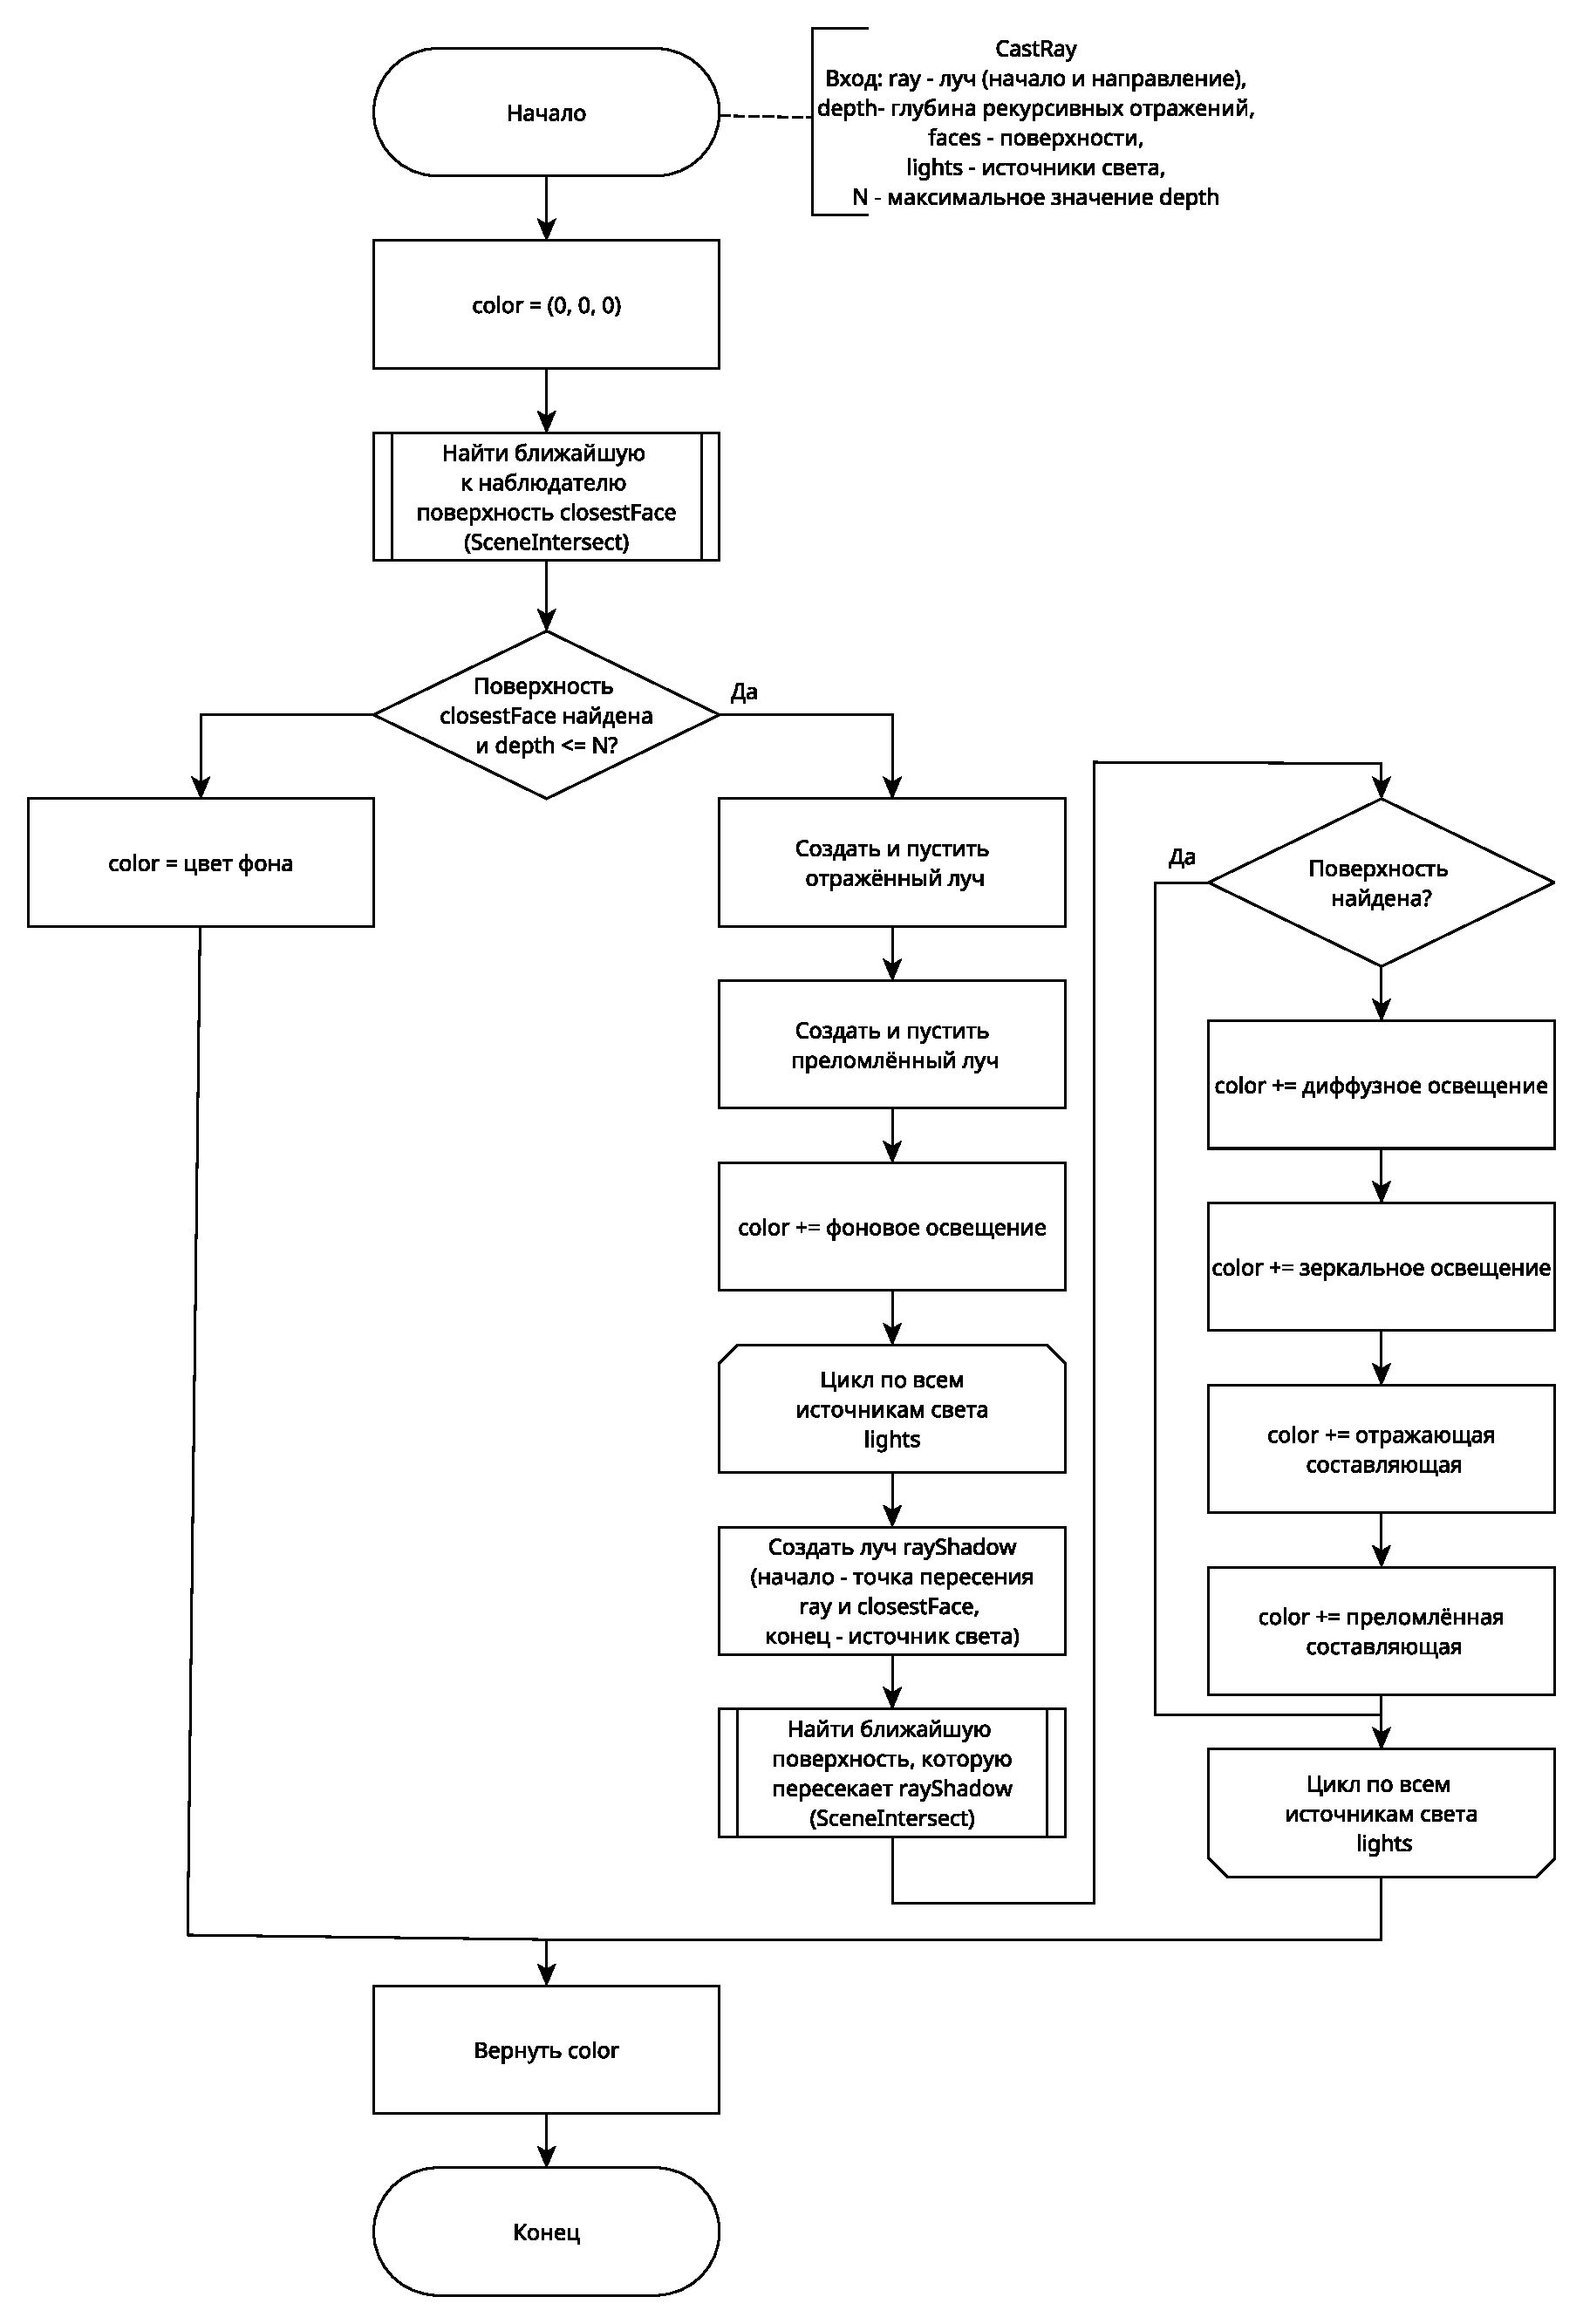
\includegraphics[width=1.0\linewidth]{include/CastRay.pdf}
		\captionof{figure}{Схема алгоритма испускания луча}
		\label{img:r1}
	\end{tabular}
\end{table}

\begin{table}[H]
	\centering
	\begin{tabular}{p{1\linewidth}}
		\centering
		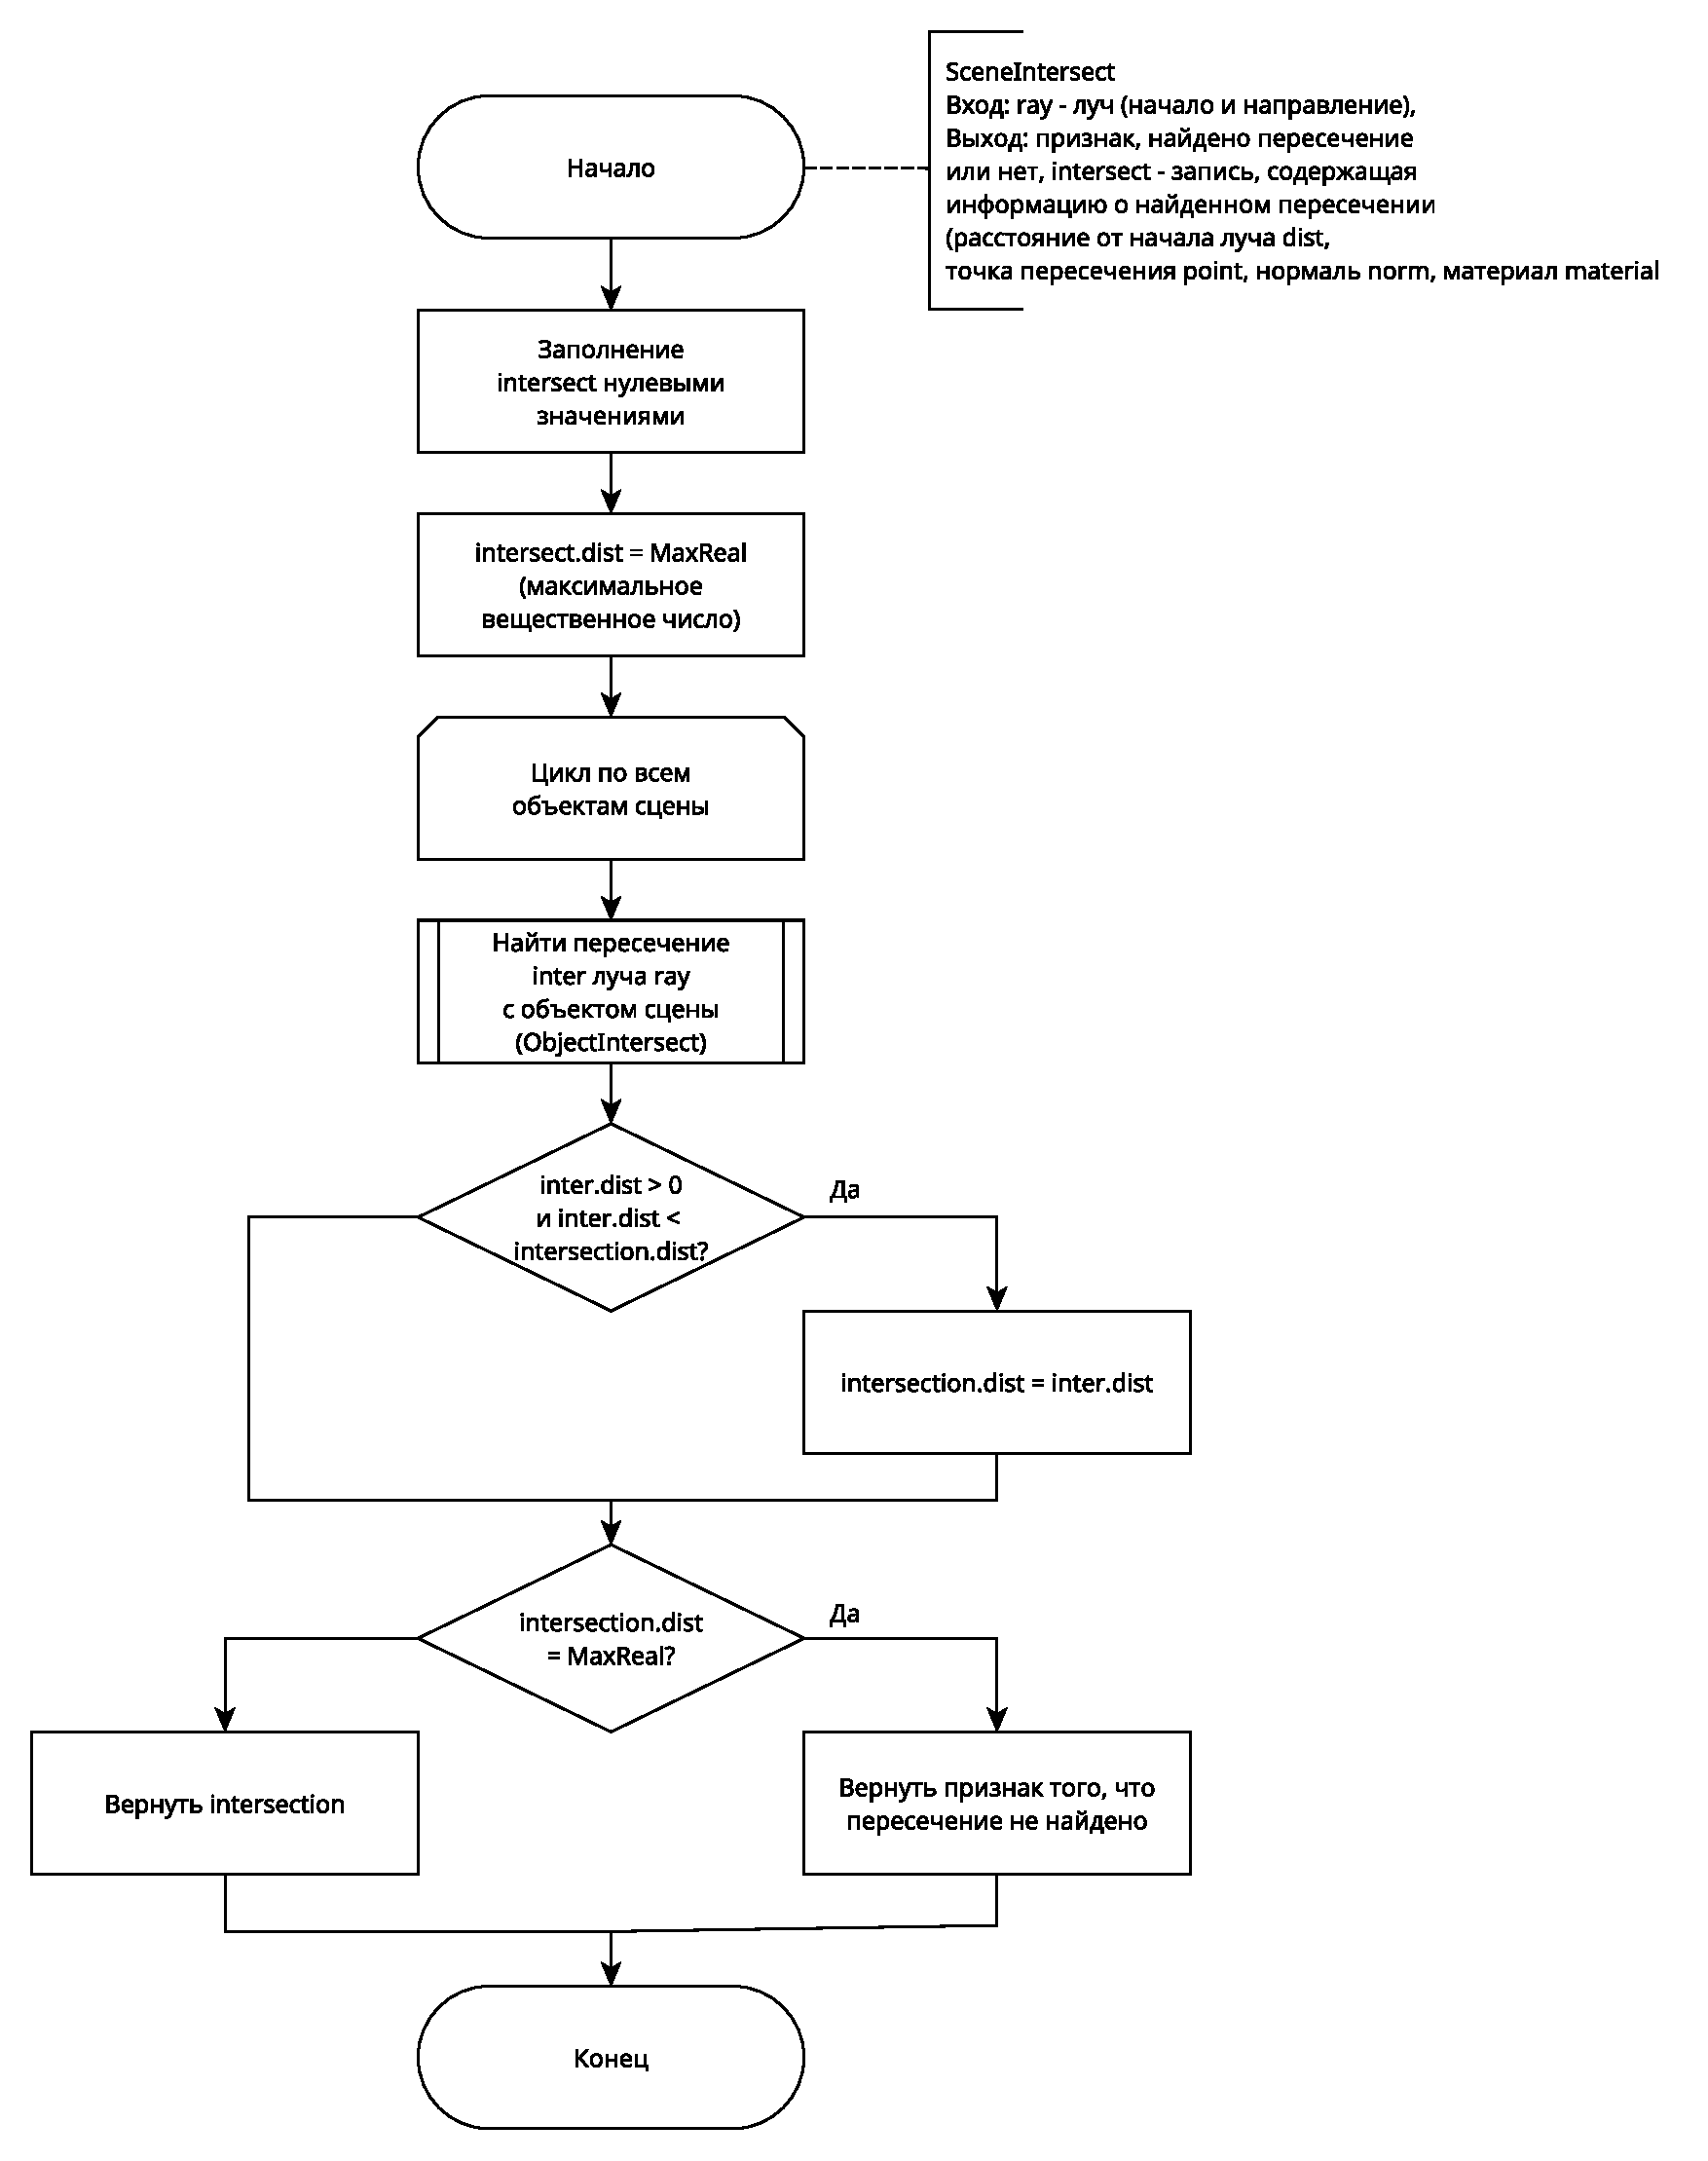
\includegraphics[width=1.0\linewidth]{include/SceneIntersect.pdf}
		\captionof{figure}{Схема алгоритма пересечения луча со сценой}
		\label{img:r2}
	\end{tabular}
\end{table}

\begin{table}[H]
	\centering
	\begin{tabular}{p{1\linewidth}}
		\centering
		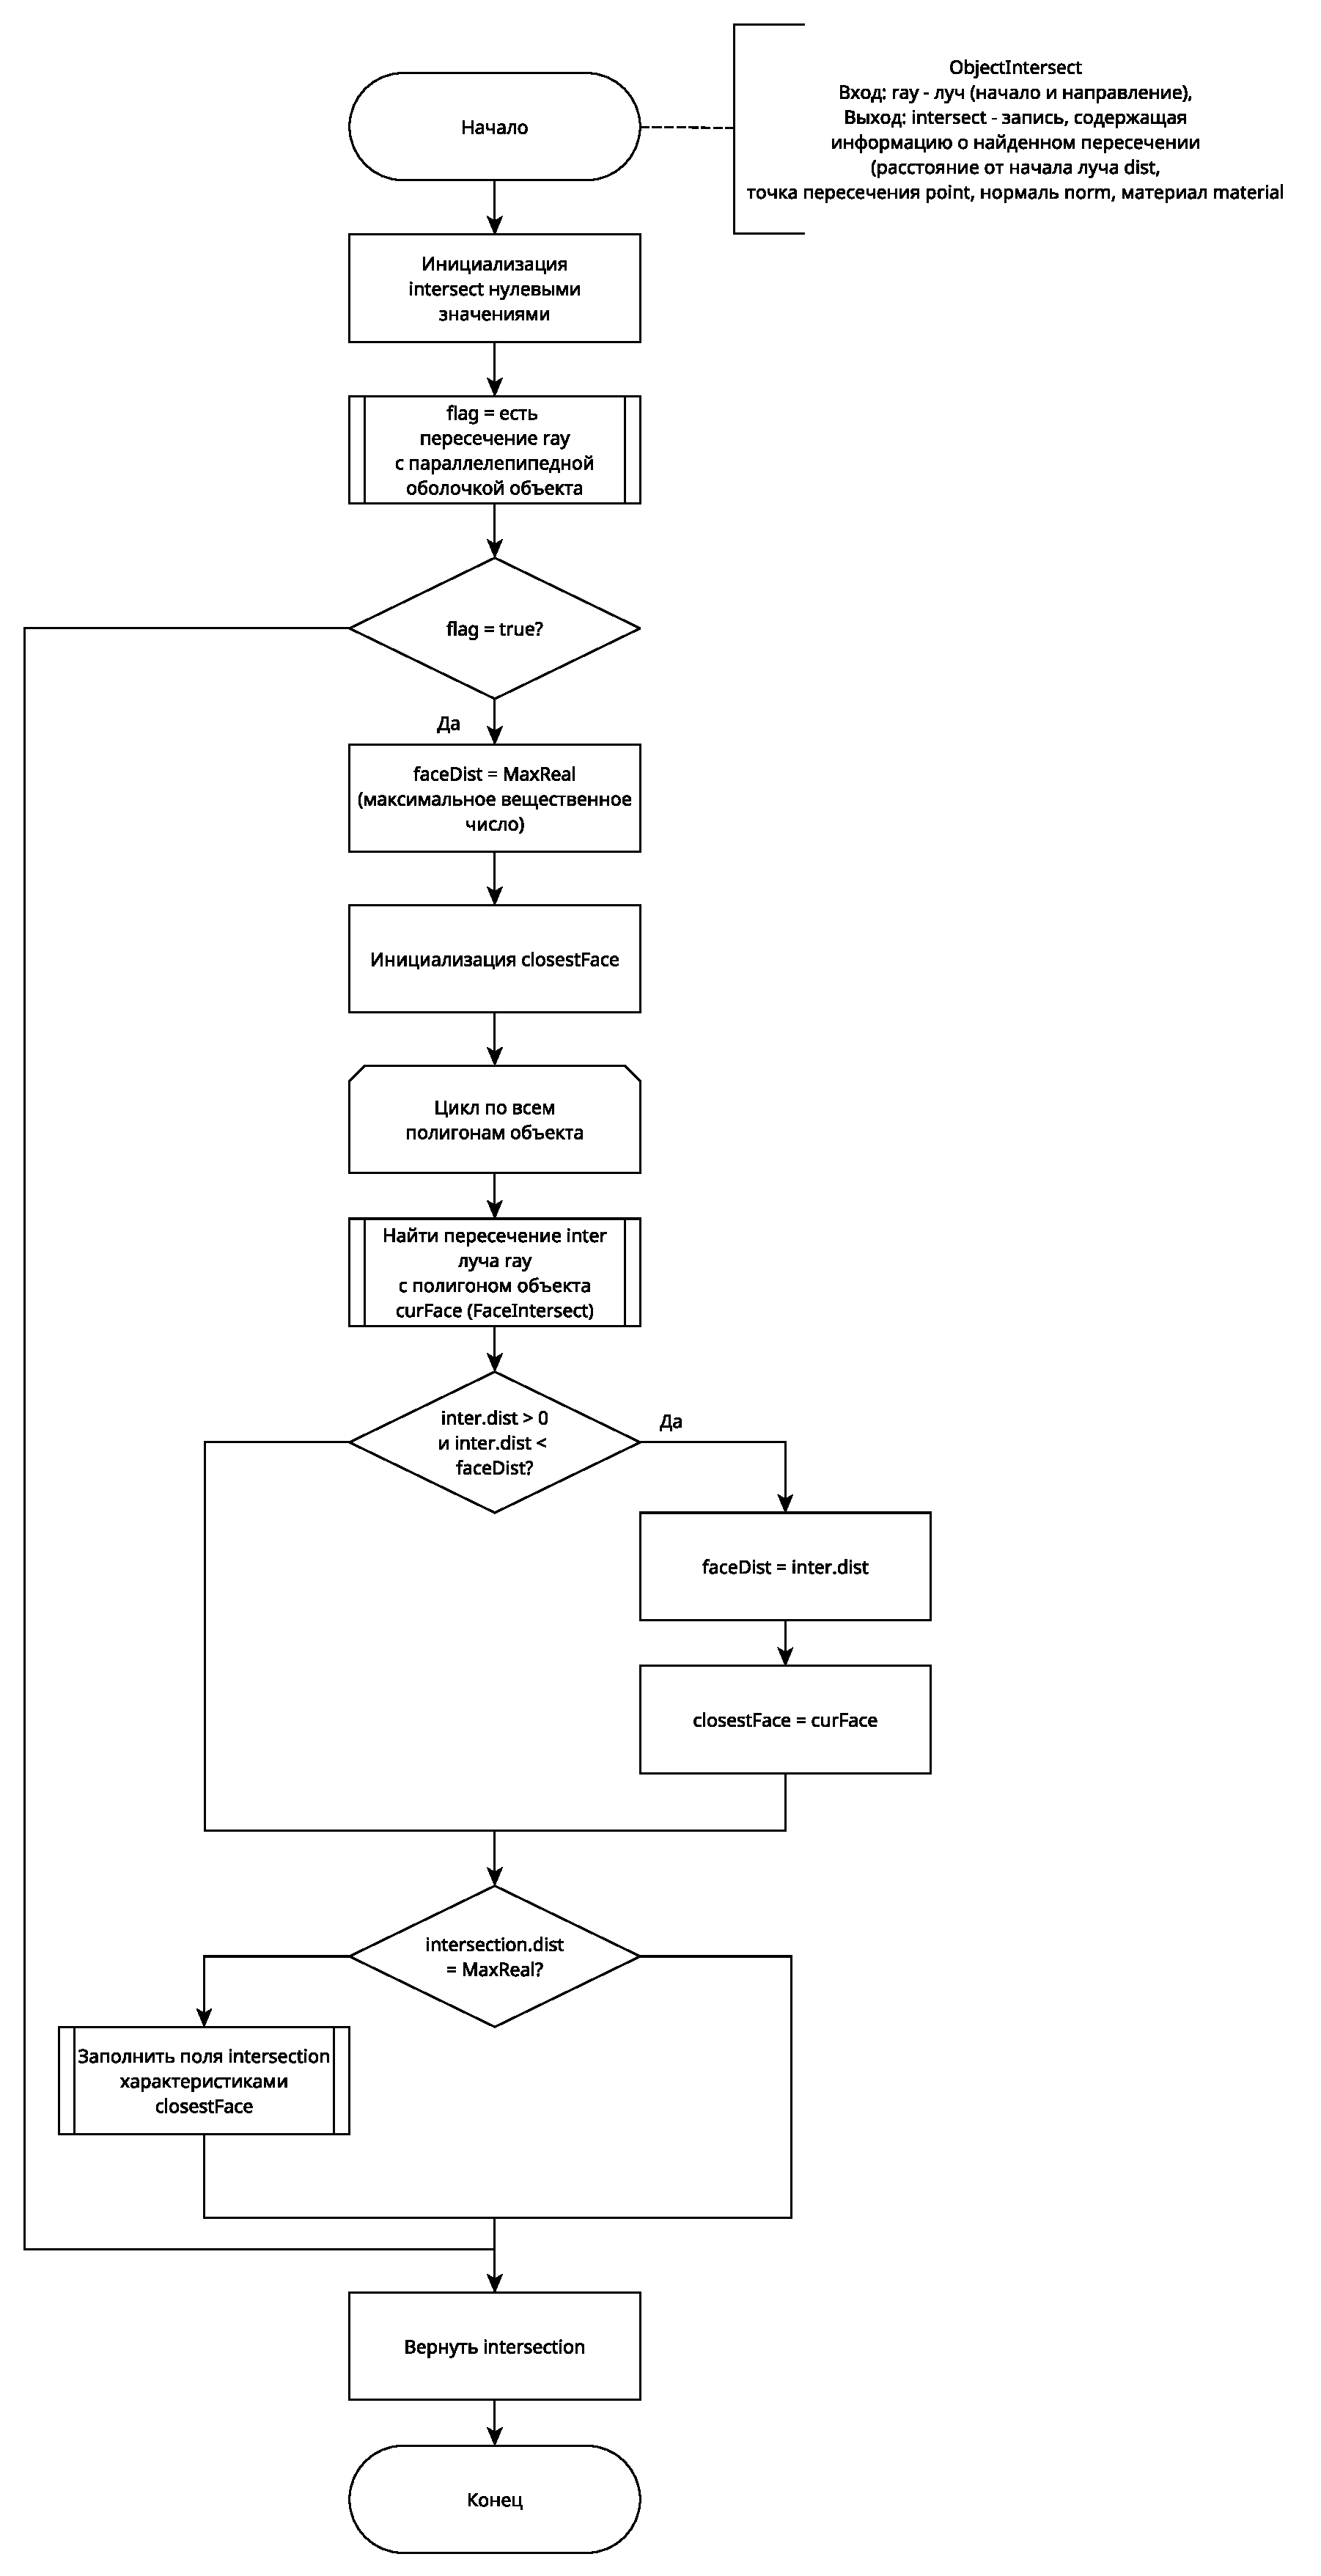
\includegraphics[width=0.75\linewidth]{include/ObjectIntersect.pdf}
		\captionof{figure}{Схема алгоритма пересечения луча с объектом}
		\label{img:r3}
	\end{tabular}
\end{table}

\begin{table}[H]
	\centering
	\begin{tabular}{p{1\linewidth}}
		\centering
		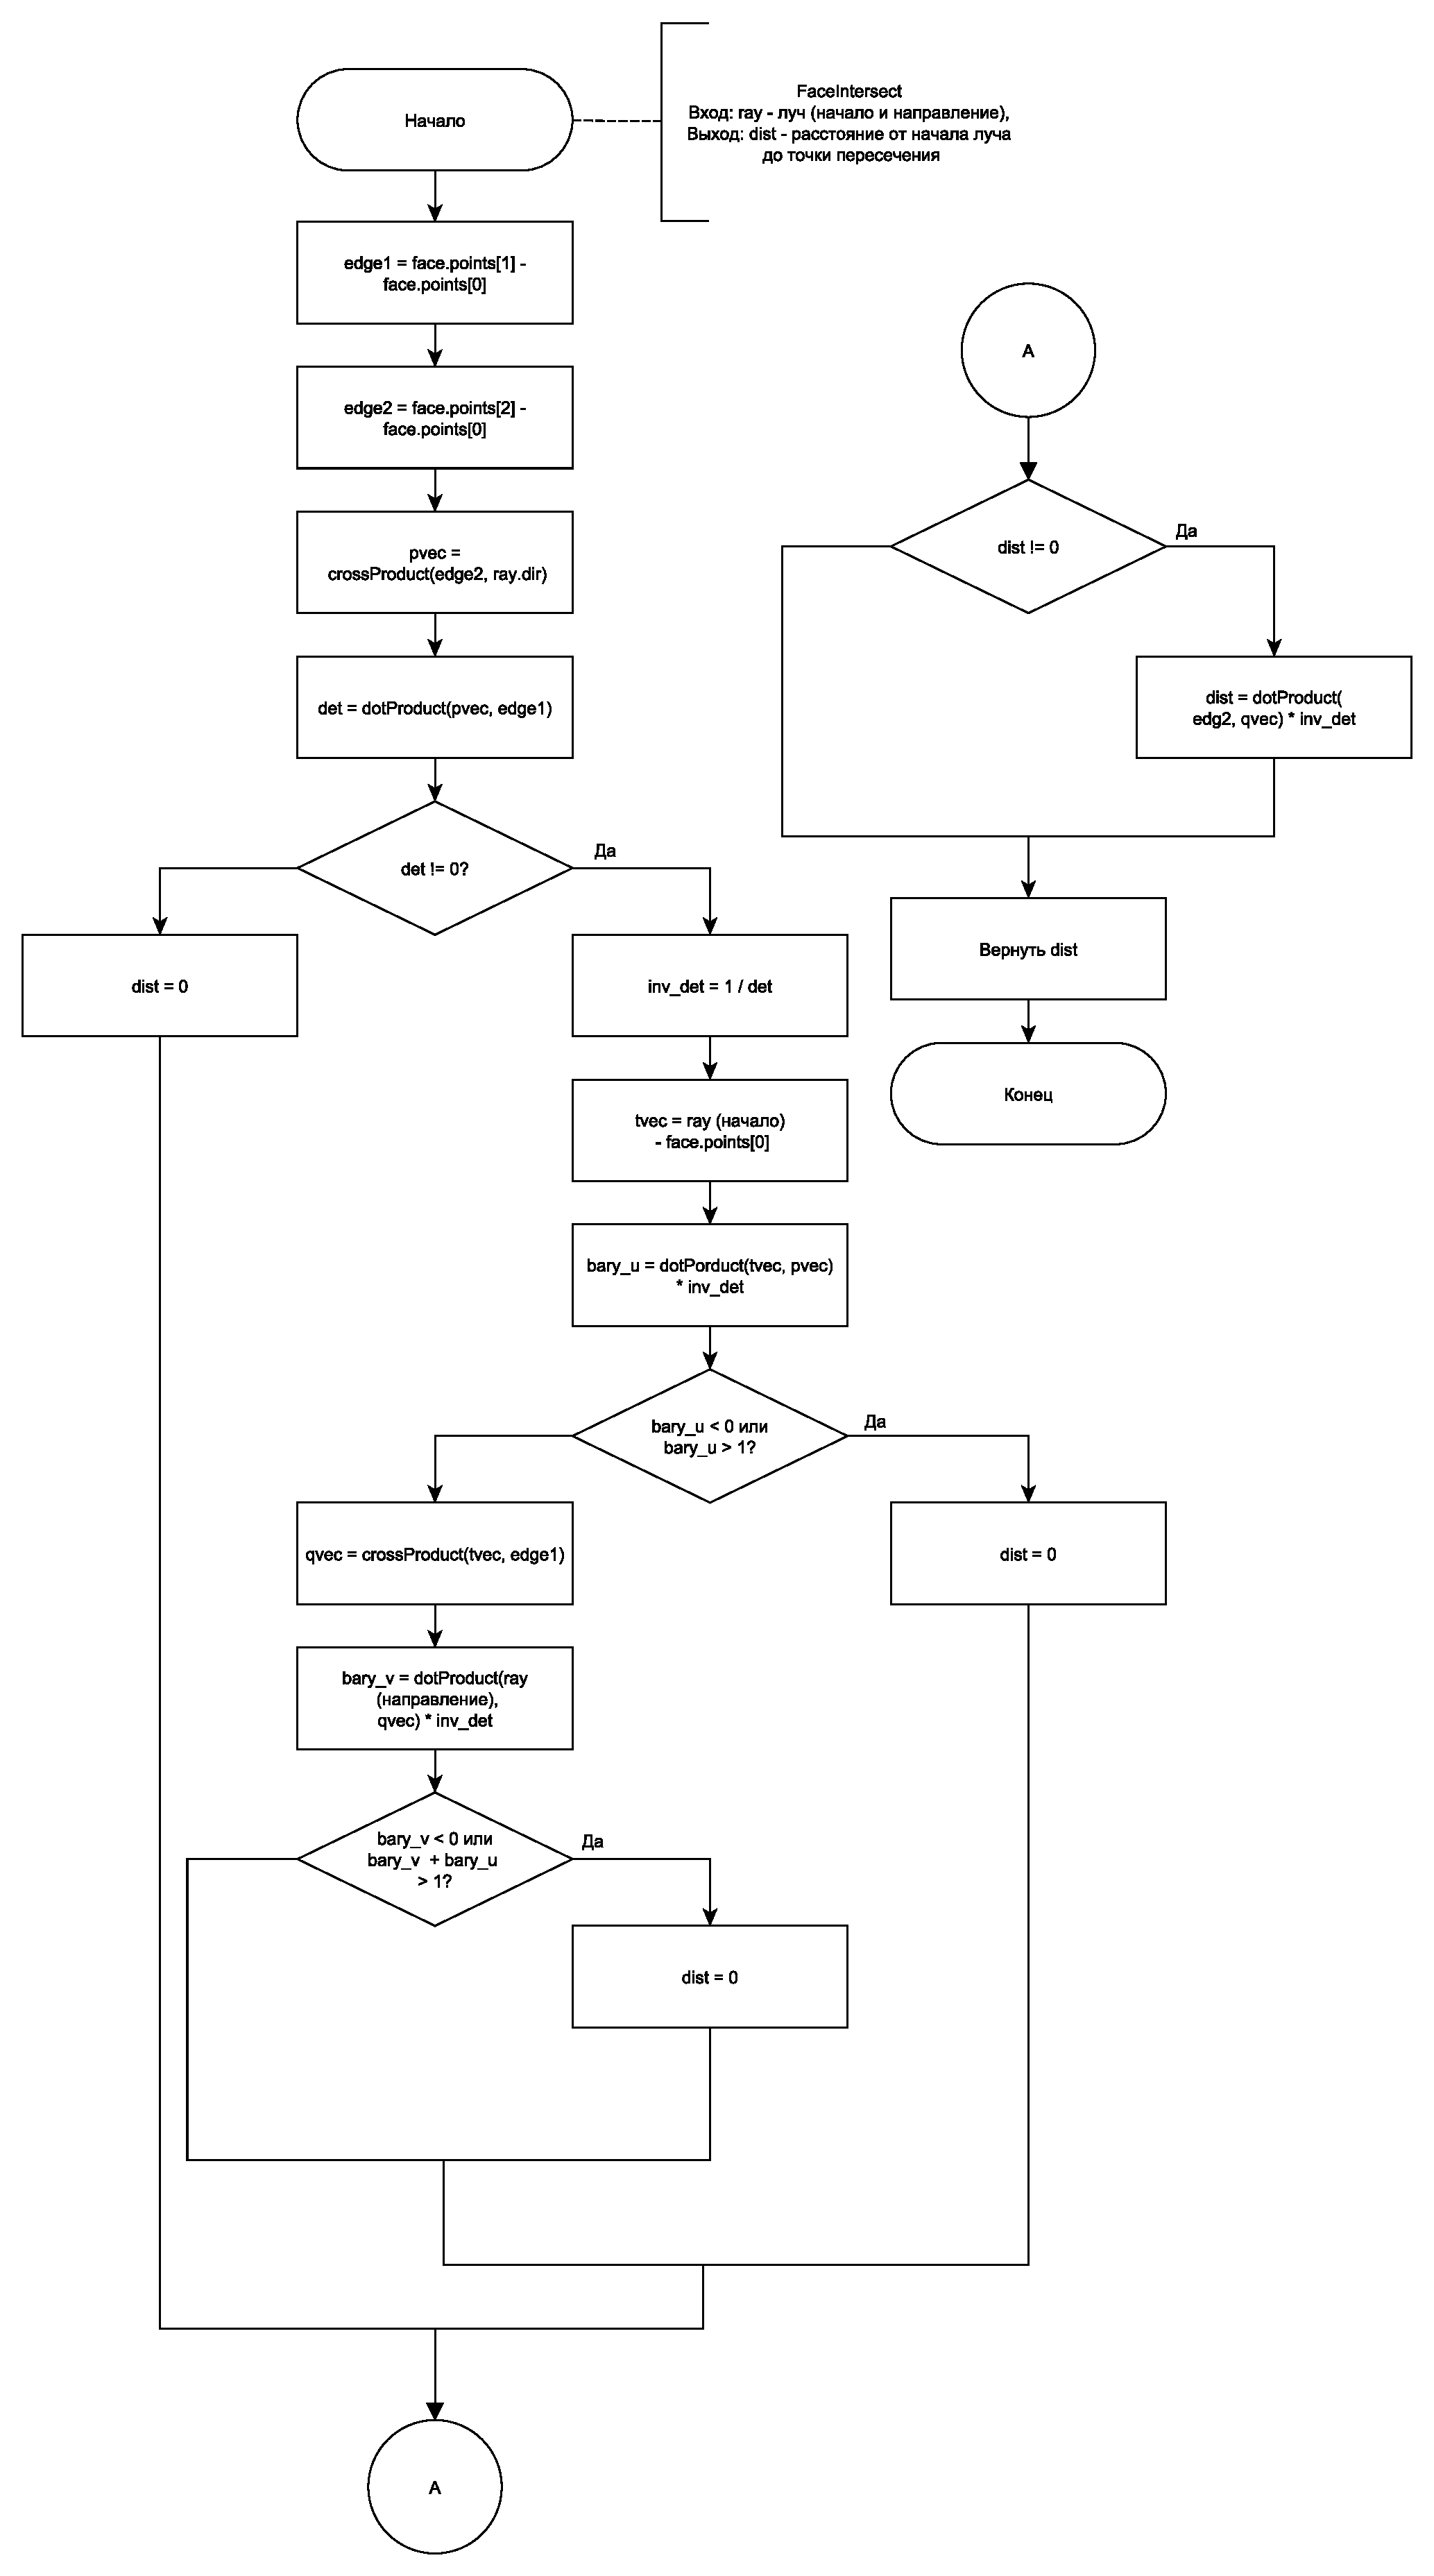
\includegraphics[width=0.8\linewidth]{include/RayFaceIntersect.pdf}
		\captionof{figure}{Схема алгоритма пересечения луча с полигоном}
		\label{img:r4}
	\end{tabular}
\end{table}

\section{Разработка типов и структур данных}\label{types}

Для формализации алгоритма синтеза изображения в программе, необходимо ввести использующиеся в ней типы и структуры данных.
\begin{enumerate}[label=\arabic*)]
	\item Структура сцены представляет собой массив с произвольным числом моделей и массив с произвольным числом источников света.
	\item Структура модели включает в себе следующие данные:
	\begin{itemize}
		\item массив вершин модели;
		\item массив полигонов модели;
		\item структуру материала модели.
	\end{itemize}
	\item Структура материала содержит в себе:
	\begin{itemize}
		\item Цвет фонового освещения (три целочисленных переменных, характеризующие цветовую модель RGB).
		\item Цвет диффузного освещения (три целочисленных переменных, характеризующие цветовую модель RGB).
		\item Цвет зеркального освещения (три целочисленных переменных, характеризующие цветовую модель RGB).
		\item Коэффициент фонового освещения (вещественная переменная).
		\item Коэффициент диффузного освещения (вещественная переменная).
		\item Коэффициент зеркального освещения (вещественная переменная).
		\item Степень, аппроксимирующая пространственное распределение зеркально отражённого света (целочисленная переменная).
		\item Коэффициент отражения (вещественная переменная).
		\item Коэффициент преломления (вещественная переменная).
		\item Показатель преломления (вещественная переменная).
	\end{itemize}
	\item Структура камеры содержит:
	\begin{itemize}
		\item Координаты положения камеры в пространстве (три вещественных переменных).
		\item Система координат камеры, задаваемая тремя ортогональными векторами.
		\item Границы пирамиды видимости (две целочисленных переменных).
	\end{itemize}
	\item Структура источника света содержит:
	\begin{itemize}
		\item Координаты положения источника света в пространстве (три вещественных переменных).
		\item Интенсивность излучения (вещественная переменная).
		\item Цвет излучения (три целочисленных переменных, характеризующие цветовую модель RGB).
	\end{itemize}
\end{enumerate}

\section{Выводы из конструкторской части}

На основе теоретических данных, полученных из аналитического раздела,
были описаны математические основы алгоритма обратной трассировки лучей, алгоритм обратной трассировки лучей,
а также было описано представление данных в программном обеспечении.
